%\hspace{24pt}

\subsection{System Model}\label{section:3.1}
%%Table1
\begin{table}[tbp]
\setlength{\belowcaptionskip}{15pt}
\centering
\caption{Notations}
\label{tab: Notations}
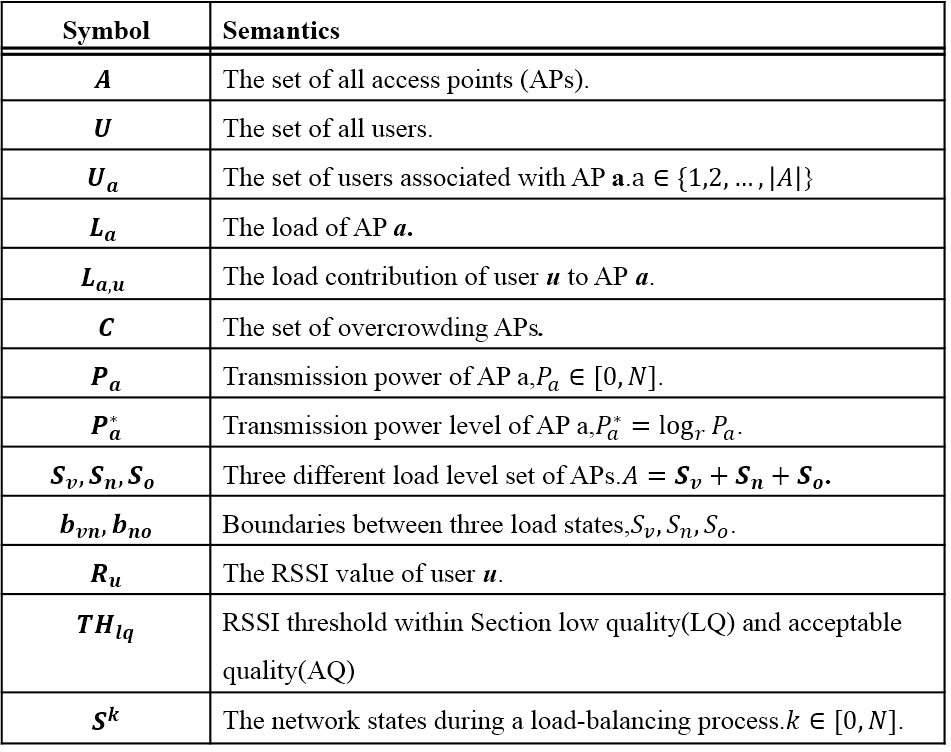
\includegraphics[width=3.4in]{images/notations.png}
\end{table}

The key notations used in our scheme are shown in Table \ref{tab: Notations}. We consider an IEEE 802.11 WLAN with a set of APs, which is denoted by $A$, and we use $|A|$ to denote the number of APs. In our system, all APs are attached to a wired infrastructure, and the distinguishing feature is that, all of them are also connected with an OpenFlow controller. Figure \ref{fig:scheme1} shows our system architecture. In our scheme, we only discuss the transmission power of AP beacon messages, because only beacon messages are related to the AP selection of users. We denote transmission power as $P_a$  . Each AP provides several transmission power levels, denoted by $P_a^*$. We define $P_a^*$ is a geometric series
\begin{eqnarray}
{P_a^*}=f({P_a})=log _r⁡\left({P_a} \right)  ,  r=\sqrt[N]{\frac{P_{max}}{P_{min}}}
\end{eqnarray}
We denote $P_a^*=P_{min}$ as the minimum power level of AP, and similarly we denote $P_N^*=P_{max}$ as the maximum power level. For normal commercial AP products, the transmission power level configuration follow that
\begin{align}
&P_k^*={P_{k-1}^*}*r\\										
&P_k^*={P_{min}^*}*{r^k}, k\in[0..N].							
\end{align}
In our scheme we have some assumptions. First, we assume that the interference between adjacent cells can be ignored. Second, we assume that the AP deployment ensures completely overlaps between the ranges of all APs. In other words, if all APs are configured to the minimum transmission power $P_{min}$, they still can cover every user in network coverage area.

When a user joins a WLAN, it listens every channel for all beacon messages from APs. Then, it associates with an AP which has strongest RSSI. The RSSI value is determined by the beacon transmission power and the distance between AP and user. In our system, we use all APs to collect the RSSIs from users  (Figure \ref{fig:scheme1}). Each AP report the RSSIs to controller by using OpenFlow protocol. Once in a while, each AP collects its load $L_a$  and the load contribution of its users $L_(a,u)$  to controller. Based on above information, the controller knows the association relationship between user and AP. In the same way, the AP loads are also known by controller. In our system, the controller has global view of the whole network.

We use $U$ to denote the set of all users in the network coverage area and let $|U|$ denote the total number of users in U. Each user associated with at most one AP at any time, and we denote $U_a$ as the set of users associated with AP $a$. In normal cases, if a large amount of user association requests are sent to an AP in a short time, the AP will overload seriously. To stress the coordination ability of APs, we consider about the group arrival cases. We assumed that all users follow a group mobility model in our system [1]. The users usually assemble in several groups and move together from one place to another.

Owing to the global vision of controller, we design an adaptive load balancing model using association allocation. Our model can coordinate the load of all the APs and take the user load contributions into consideration. We consider busy users that use all the allocated bandwidth, i.e. they always upload or download data. Controller records the load contribution $L_{a,u}$ of user $u$ to AP a by considering the load report from APs. Each AP can provide different bandwidth to its associated users in our case.

%% Figure 3.1

\begin{figure}[tbp]
\begin{center}
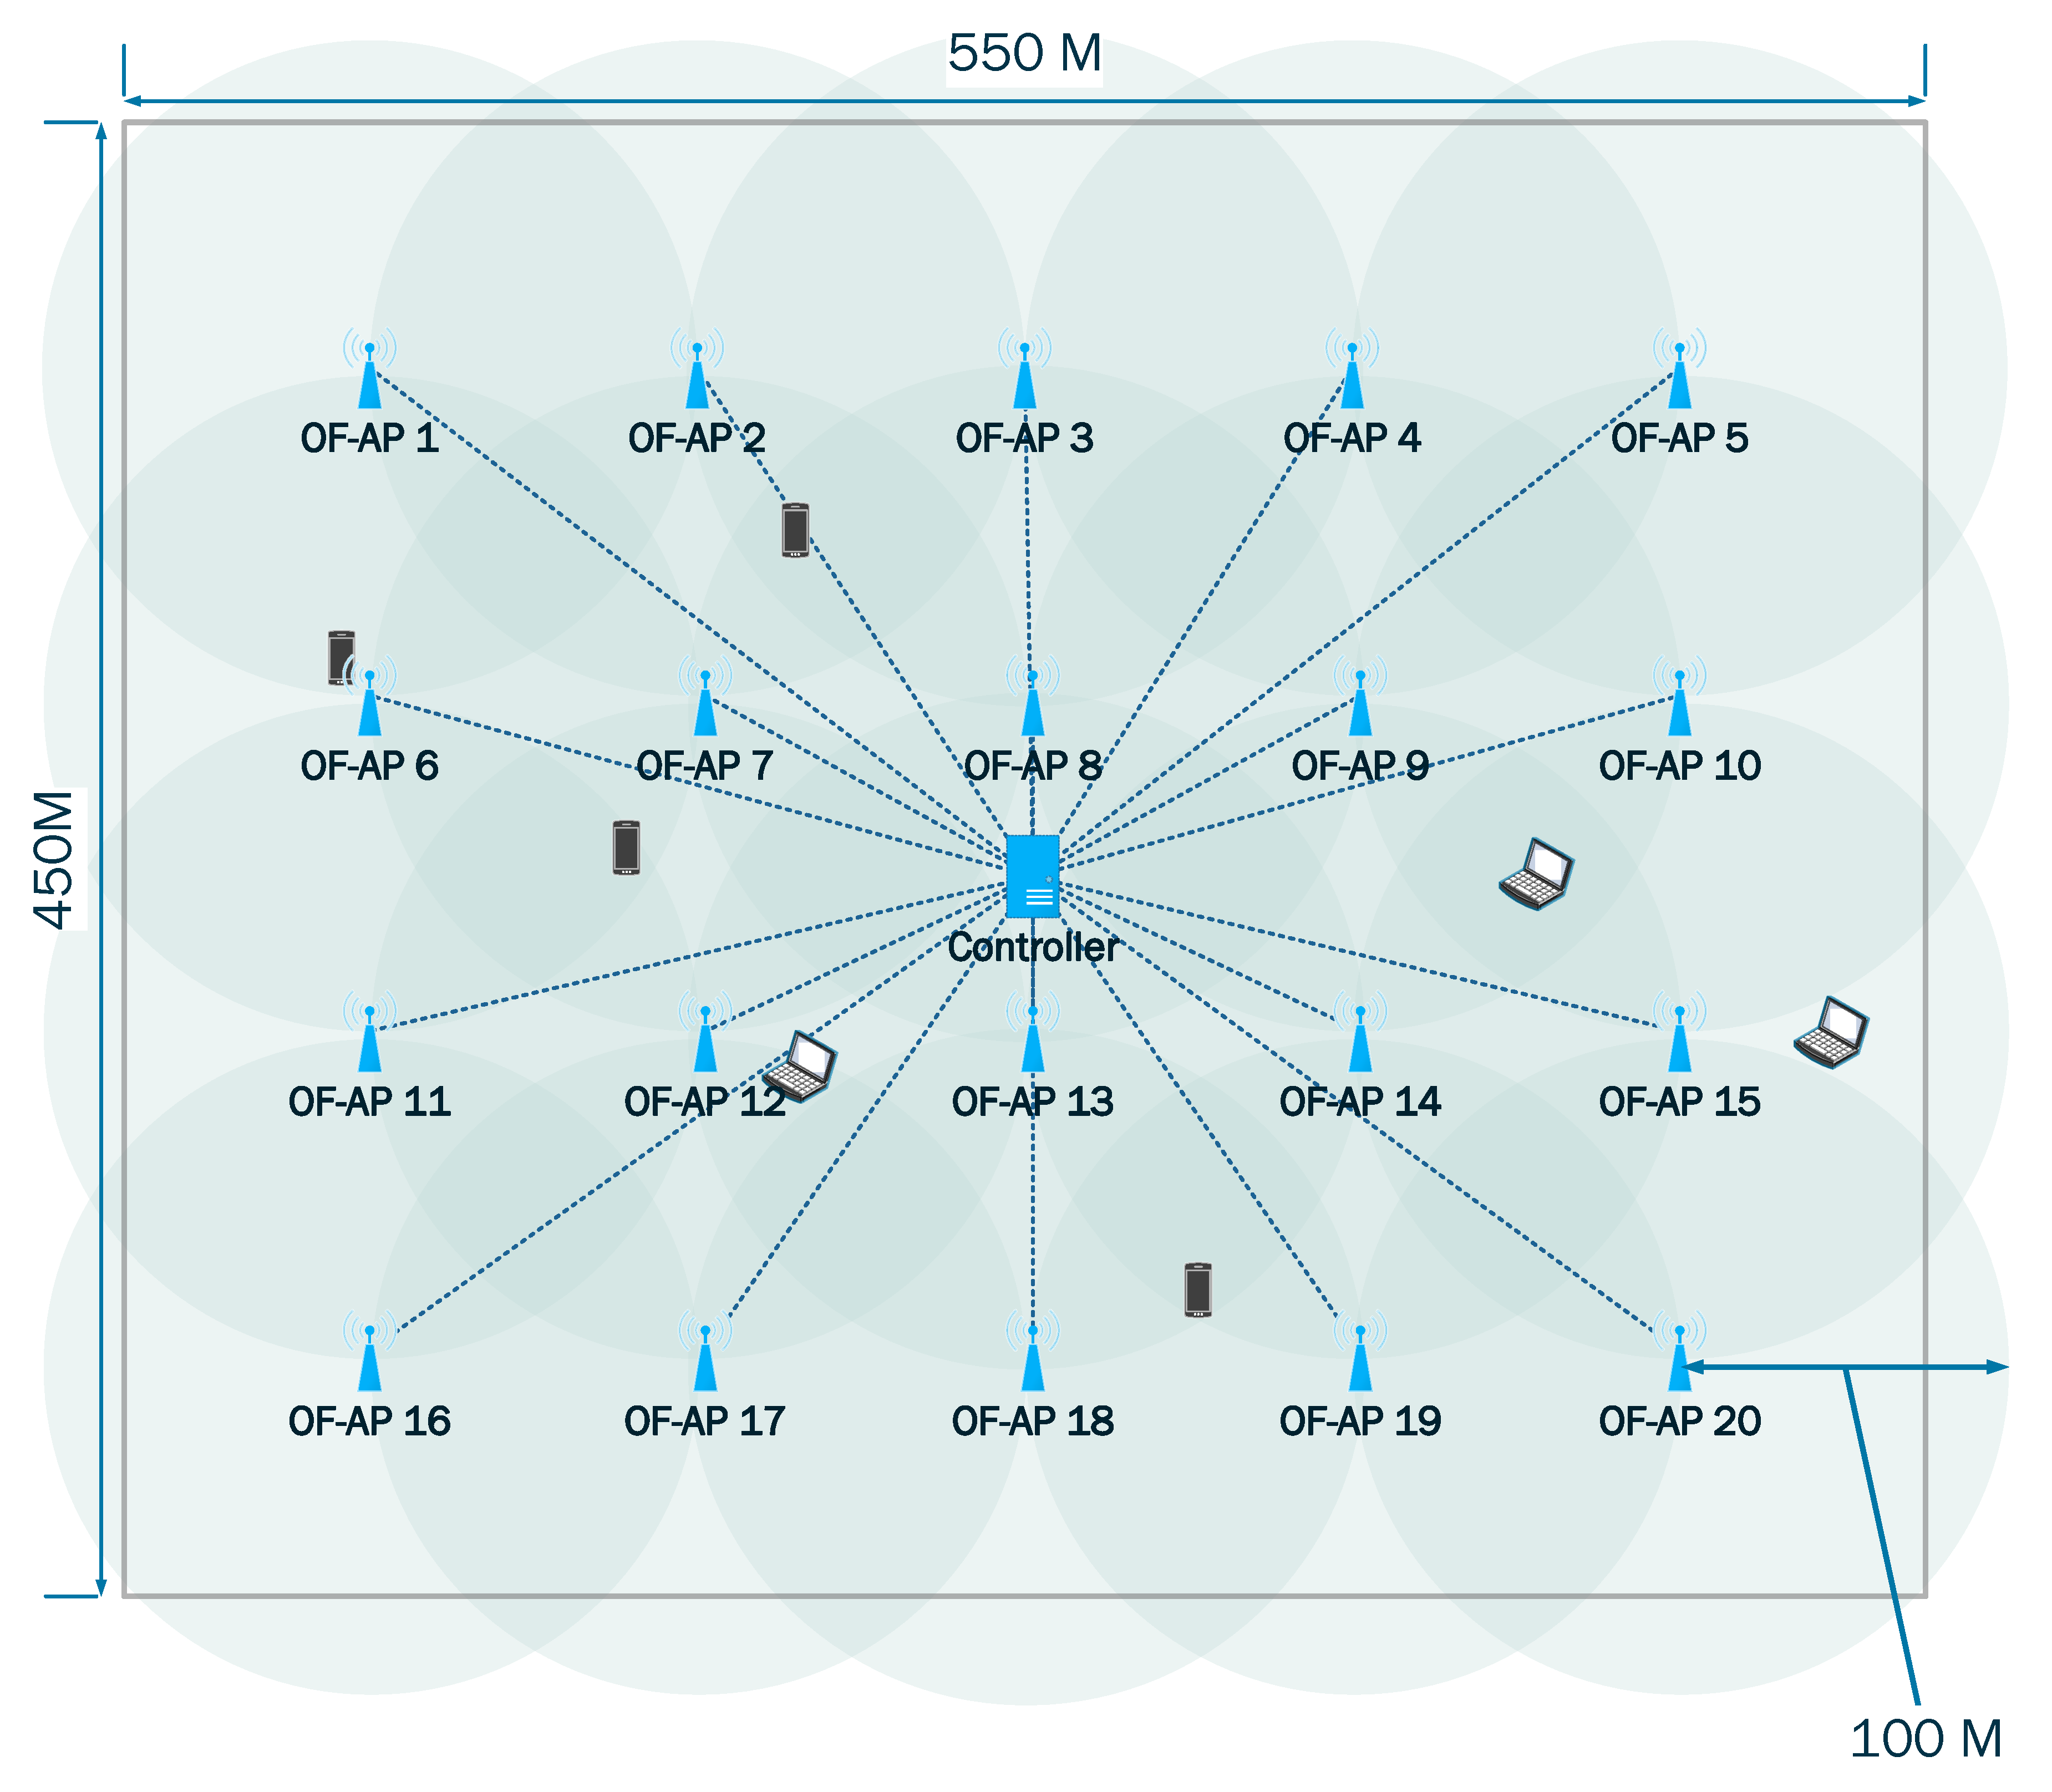
\includegraphics[width=3.4in]{images/scheme1.pdf}
\end{center}
\caption{System Architecture}
\label{fig:scheme1}
\end{figure}
%\clearpage

\subsection{Arrival Event Detection}\label{section:3.2}
In this subsection, we present the initial stage of adaptive load balancing. We design each AP to report its user association event and load in real time. Figures \ref{fig:flowdiagram_trendindicator_ap} and \ref{fig:flowdiagram_trendindicator_controller} show the flow diagram of AP report transmission and controller manage mechanism, respectively.
\begin{description}
  \item [Step 1.] Each AP records the user RSSI, user association list and its load periodically. All APs receive RSSIs in every authentication frames from their users.
  \item [Step 2.] To inspect whether a new user associates with the AP successfully or not. If the AP sends association response (Success) to user, it means that a new association is established.
  \item [Step 3.] The AP sends the user’s RSSI to the controller. Then go to \textbf{Step 6}.
  \item [Step 4 and 5.] If there is no new arrival in Step 2, the AP reports its load to controller periodically.
  \item [Step 6.] After sending report messages to controller, the AP would receive a response message from controller. Upon receipt of the Beacon-Config message, the AP configures its beacon transmission power accordingly in \textbf{Step 7}.
  \item [Step 7.] The AP configures its beacon power.
\end{description}

%% Figure 3.2
\begin{figure}[tbp]
\centering
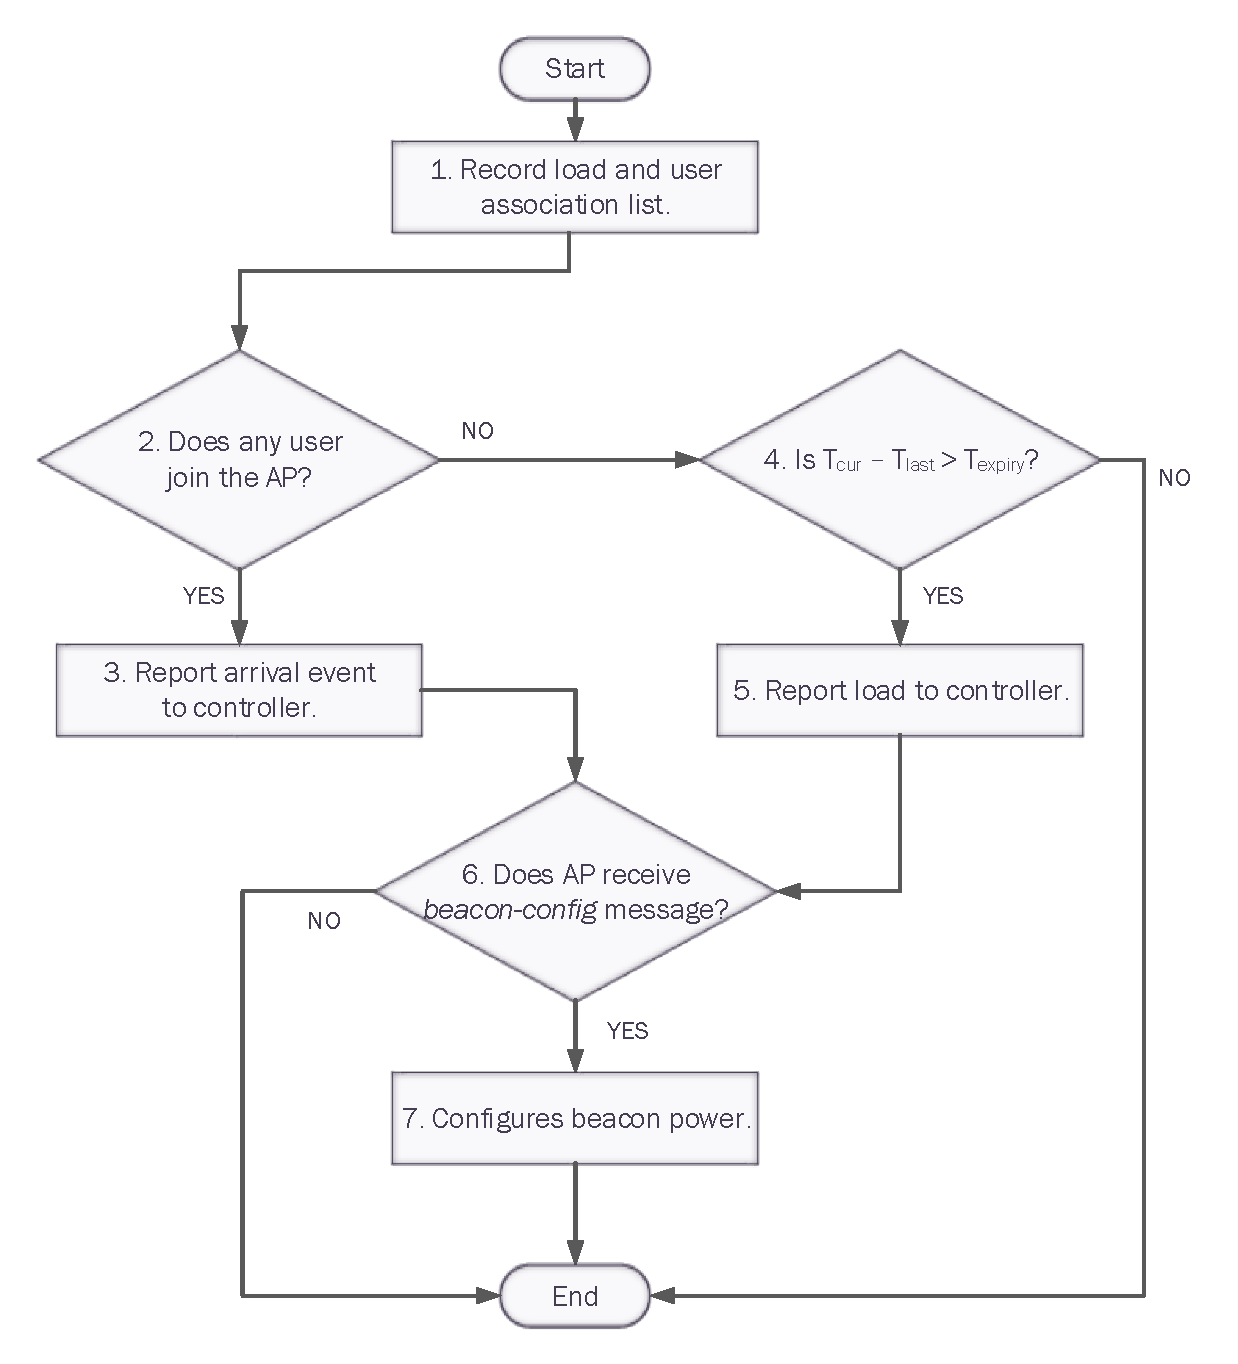
\includegraphics[width=3.4in]{images/flowdiagram_trendindicator_ap.pdf}
\caption{Flow Chart for AP Report Mechanism}
\label{fig:flowdiagram_trendindicator_ap}
\end{figure}

%\clearpage

On the other side, we describe a flow chart of controller manage mechanism in Figure \ref{fig:flowdiagram_trendindicator_controller}.

\begin{description}
  \item [Step 1.] The controller receives arrival events and load messages from APs.
  \item [Step 2.] Add new arrival events into the arrival count tables. Then calculate the number of event increase in latest time interval.
  \item [Step 3.] The controller compares the number of current arrival events with the past. If the tendency to increase of an AP exceeds a threshold, that means the AP has a high risk of overcrowding, the controller would give the AP a predicted load value and then run load balancing algorithm (\textbf{Step 6}).
  \item [Step 4.] The controller classifies all APs into three load levels, which are vacant, normal and overcrowding. We define three set of APs $({S_v}, {S_n} and {S_o})$, and let $b_{vn}$  and $b_{no}$ denote the boundaries between these levels.

      \begin{align}
        &L_(l,a)=\left\{\begin{array}{rcl}
            v, L_a≤b_{vn} \\ n, L_a≤b_{no} \\ o, L_a<b_o
            \end{array} \right\} \\
            \nonumber\\
        &S_v={a|L_(l,a)=v}\\
        &S_n={a|L_(l,a)=n}\\
        &S_o={a|L_(l,a)=o}
      \end{align}
  \item [Step 5.] Check whether any AP change to overcrowding state $S_o$.
  \item [Step 6.] Run load balancing algorithm. We will mention the load balancing algorithm in next subsection.
  \item [Step 7.] After the load balancing procedure, the controller send a beacon-config messages to each AP.
\end{description}

%% Figure 3.3
\begin{figure}[tbp]
\begin{center}
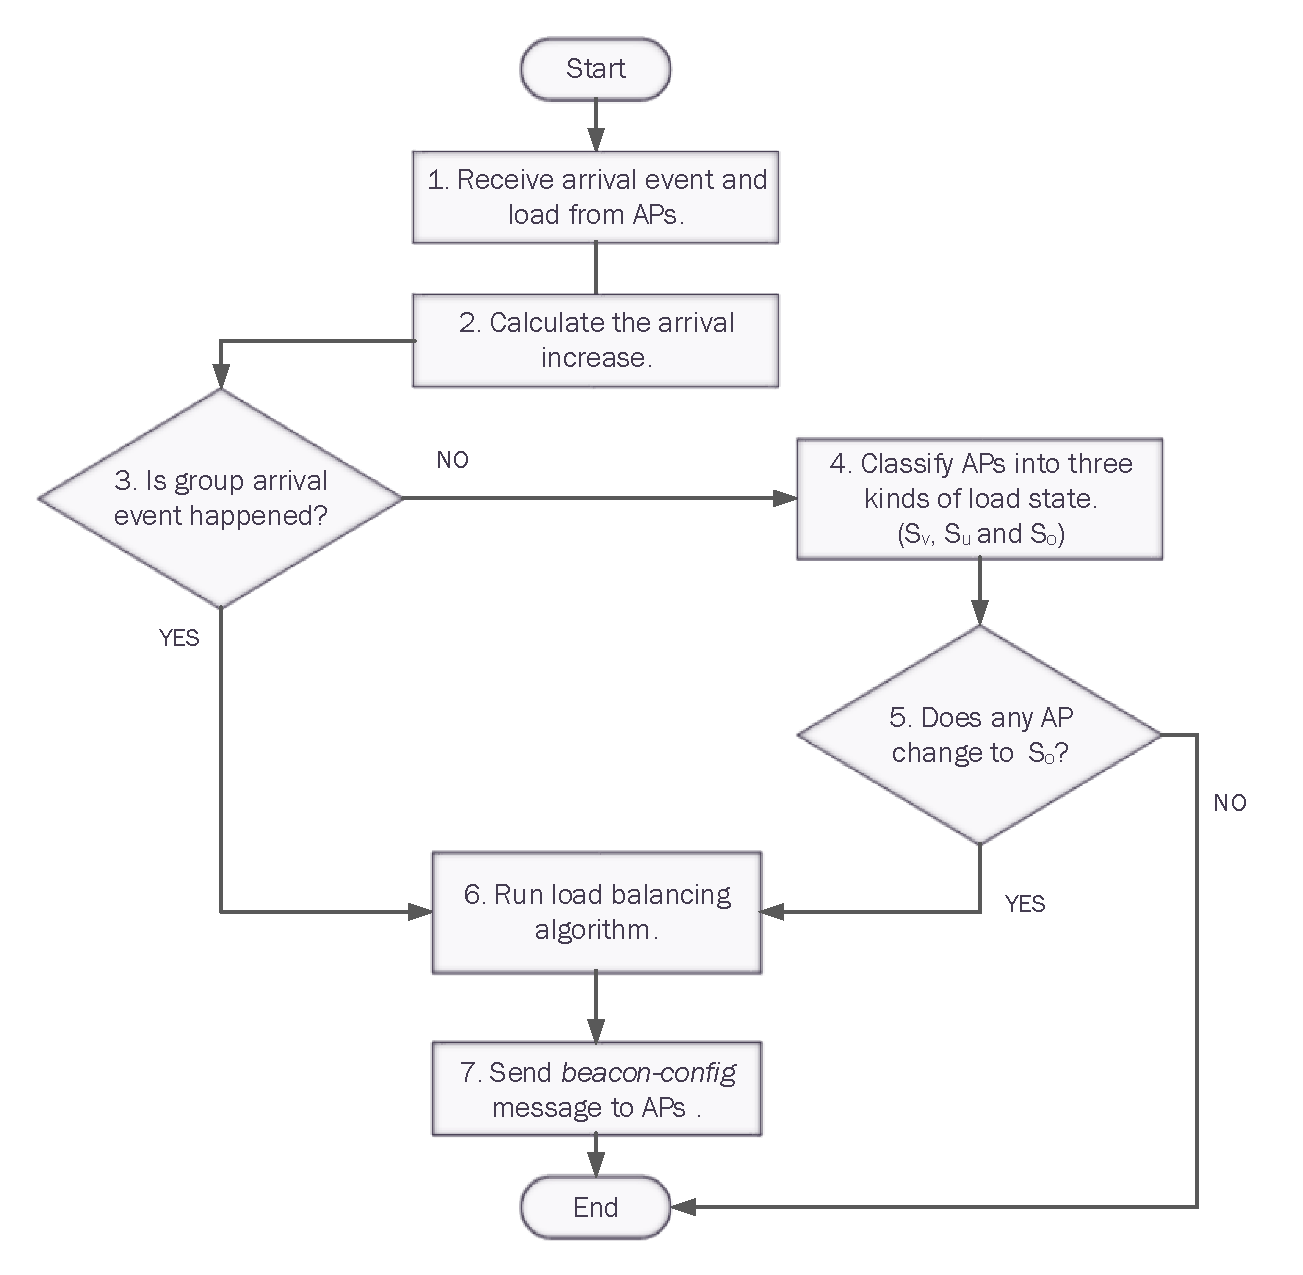
\includegraphics[width=3.4in]{images/flowdiagram_trendindicator_controller.pdf}
\end{center}
\caption{ Flow Chart for Controller Manage Mechanism}
\label{fig:flowdiagram_trendindicator_controller}
\end{figure}
%\clearpage

\subsection{Adaptive Load Balancing}
In this subsection, we present the adaptive load balancing mechanism. Recall that we described in subsection \ref{section:3.1} and \ref{section:3.2}, the association relationship, RSSIs of users and load of APs are all collected by the controller. Thanks to the above knowledge, the controller has global vision of whole wireless network. We combine SDN and Cell-Breathing method into an Adaptive Load Balancing mechanism.

 Figure \ref{fig:algorithm} shows the pseudo code of our mechanism for controller. In this algorithm, the beacon power level is first initialized to the maximal power level. The controller collects and calculates the summation of all AP utilizations, and it is initialize as state $S^0$. First, the algorithm iteratively finds the most overcrowding AP, then set its power one level down. In the meanwhile, the adjustment is recorded in a stack structure and the most overcrowding AP is added into overcrowding set $C$. After setting down beacon power level each time, the algorithm updates the AP states by simulating the association relationship between APs and users. Each state is compared with previous states to find the optimal state. Until the iteration ends, the algorithm sets all AP beacon power level according to the optimal state.

This algorithm terminates in two conditions. The first condition is that the overcrowding set $C$ is equal to AP set $A$. If these two set are equal, that means all the APs are adjusted a round. If the iteration continues, there are more rounds and the results are the same. The second condition checks whether any AP beacon power level is zero. If the iteration continues, some of the APs can not trun down their beacon power anymore, thus they will become overcrowding again.

%% Algorithm
\begin{figure}[tbp]
\centering
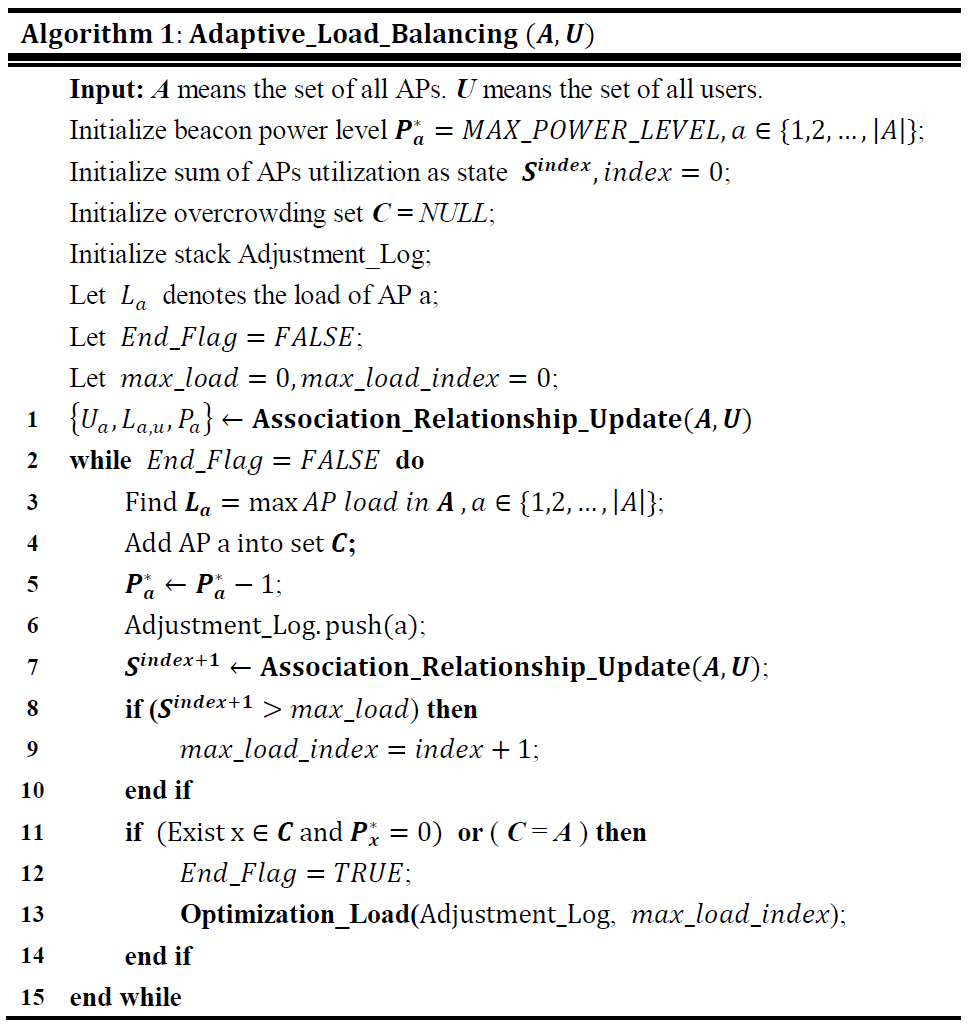
\includegraphics[width=3.4in]{images/algorithm.png}
\caption{Adaptive Load-Balancing Algorithm}
\label{fig:algorithm}
\end{figure}
%\clearpage

Figure \ref{fig:flowchart_Cell_Breathing} illustrates the message flow of association control between user, APs and controller. We assume that user is in the coverage of AP 1 and 2, and AP 1 is closer to user than AP 2. We assume that the user has passwords of AP 1 and 2. Both these two APs connect to controller via secure channel.

\begin{description}
  \item [Step 1.] AP 1 and AP 2 send Beacon Message to user periodly.
  \item [Step 2.] AP 1 and AP 2 report their load (utilization) and association events to controller. In OpenFlow protocol, association event can be transmit in Packet\_In message and the AP load information can be transmit in Port\_Status message.
  \item [Step 3.] Controller periodly checks all the AP loads and association and integrates all association event reports of APs. Then controller inputs these information to Adaptive Load Balancing program.
  \item [Step 4.] Based on the result of \textbf{Step 3}, controller sends Beacon-Config messages (i.e. SetConfig message in OpenFlow) to APs. In this case, controller decides to reduce AP 1 load, thus controller sets the AP 1 beacon power lower than AP 2 beacon power.
  \item [Step 5.] The same as \textbf{Step 1}, AP 1 and AP 2 send beacon message to the user.
  \item [Step 7-9.] The user sends association request to AP 2, which has the highest RSSI(Received Signal Strength Indicator) value. After receiving association response form AP 2, user sends authentication request to AP 2. If AP 2 sends back authentication response, the connection between user and AP 2 is established.
\end{description}

%% Figure 3.4
\begin{figure}[tbp]
\begin{center}
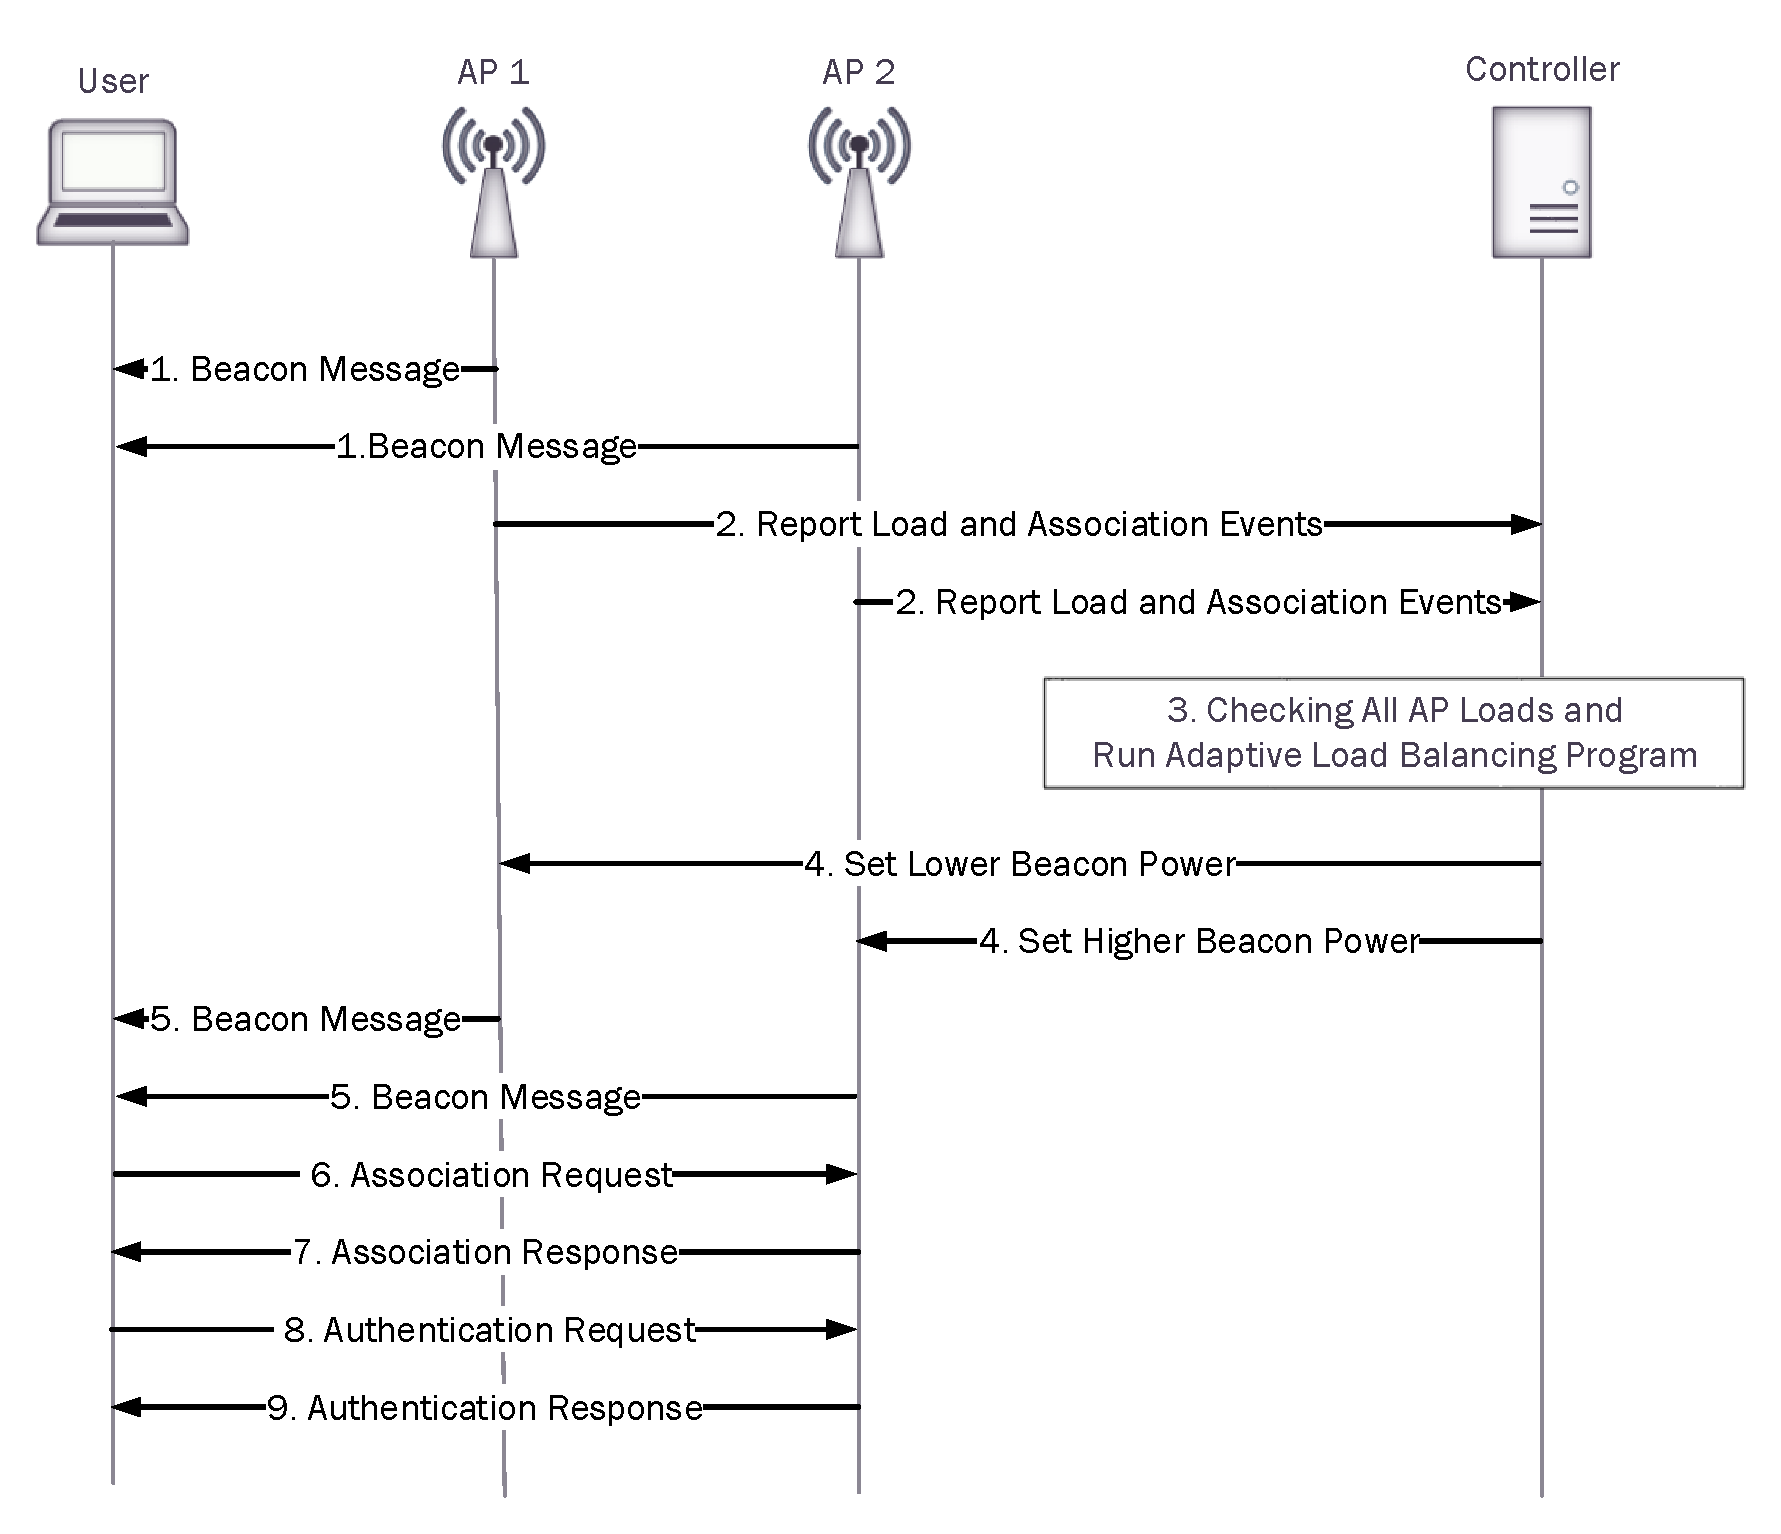
\includegraphics[width=3.4in]{images/flowchart_Cell_Breathing.pdf}
\end{center}
\caption{Message Flow of Association Control}
\label{fig:flowchart_Cell_Breathing}
\end{figure}

% above Dotto


